\section{强化学习简介}
强化学习(Reinforcement Learning)这一名词来源于心理学。俄国心理学家\citeauthor{pavlovConditionedReflexesInvestigation1927}在\citeyear{pavlovConditionedReflexesInvestigation1927}年发表的《\citetitle{pavlovConditionedReflexesInvestigation1927}》中用“强化”(reinforcement)一词描述特定刺激使生物趋于采取某种策略的现象,相应的刺激称为“强化物”(reinforcer)\cite{pavlovConditionedReflexesInvestigation1927}。在后续的研究中,心理学家将强化分为正强化(positive reinforcement)和负强化(negative reinforcement),其中正强化使得生物趋于做出能够获取更多利益的行为,而负强化则使其避免损害\cite{michaelPositiveNegativeReinforcement1975}。

% 生物的这一特性为人工智能领域的研究者提供了灵感,他们据此提出了强化学习的概念。在一个强化学习系统中,代理(Agent)可以观察环境,根据其决策策略(Policy)做出行动(Action)。在行动之后获得奖励(Reward)。强化学习即是通过与环境的交互学习如何获取最大化奖励的过程\cite{xiao2019}。因此,一个强化学习系统具有两个关键元素:奖励和策略。

% 奖励是强化学习系统学习的目标,代理在行动后总会接收到环境发来的奖励,这一奖励与心理学中的强化物对应,包括正奖励和负奖励。代理会根据观测情况决定采取不同的动作,这种从观测到动作的映射关系即为策略。系统通过改进策略获得奖励的最大期望值,因此,强化学习的学习对象即为代理的策略。策略既可以是确定性的,也可以是不确定性的。

% 基于强化学习的人工智能已经在电子游戏竞技、棋盘类游戏及自动驾驶等领域有了非常成功的应用,图\ref{figure_rldemo}列举了其中部分成果。
% \begin{figure}[htbp]
%   %\vspace{13pt}
%   \centering
%   \subfigure[在电子游戏spaceinvader中应用强化学习\cite{volodymyrHumanlevelControlDeep2015}]{\label{figure_rldemo_game}
%   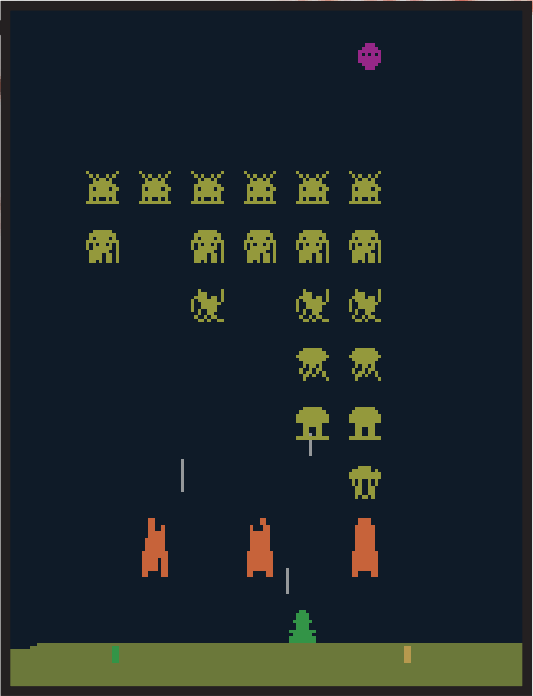
\includegraphics[height=0.23\linewidth]{images/ch04/spaceinvader.png}
%   }\hspace{0.05\linewidth}
%   \subfigure[AlphaGo Zero学习的一盘棋局\cite{silverMasteringGameGo2017}]{\label{figure_rldemo_go}
%   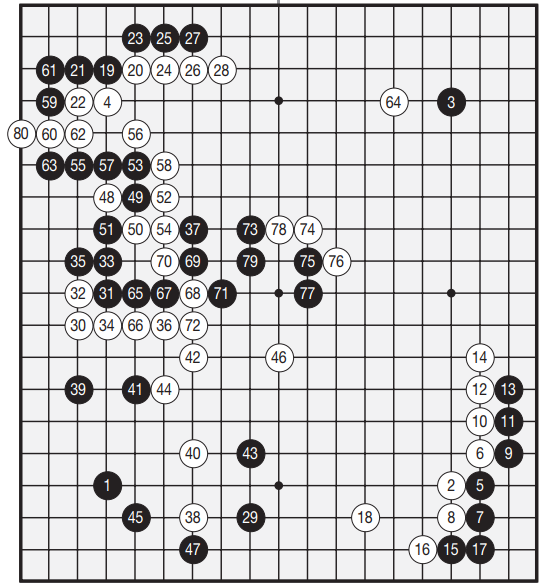
\includegraphics[height=0.23\linewidth]{images/ch04/alphazero.png}
%   }\hspace{0.05\linewidth}
%   \subfigure[AirSim仿真平台中应用强化学习实现自动驾驶\cite{wuNavigatingAssistanceSystem2018}]{\label{figure_rldemo_auv}
%   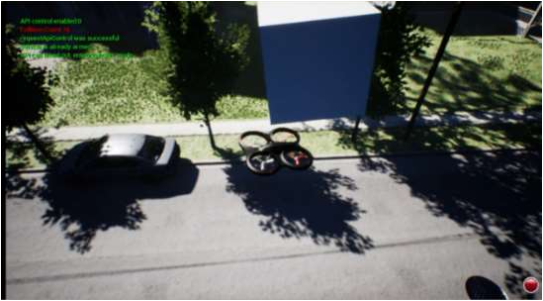
\includegraphics[height=0.23\linewidth]{images/ch04/airsim.png}
%   }
%   \caption{部分强化学习应用场景}\label{figure_rldemo}
% \end{figure}
% 在图\ref{figure_rldemo}\subref{figure_rldemo_game}中,研究者利用深度Q学习算法(DQN)进行训练,其状态根据敌人占据游戏屏幕的情况划分。在经过$2~h$训练后,这一系统“学习”到当敌人占满屏幕后将会导致游戏失败,因此采取了与人类相似的行为规避\cite{volodymyrHumanlevelControlDeep2015}。2016年,DeepMind的强化学习系统AlphaGo击败围棋选手李世石受到公众广泛关注,随后开发的智能程序AlphaZero不仅能从人类棋谱中学习如何在围棋竞技中获胜,并且完成自我对弈,采用这种方式训练的AlphaZero能在对局中击败AlphaGo\cite{silverMasteringGameGo2017},展示出强化学习强大的学习和进化潜力。除此以外,利用深度强化学习训练的自动驾驶系统具有较强的反应和修正能力\cite{wuNavigatingAssistanceSystem2018},相关研究正在迅速发展壮大。

% 强化学习的目标为寻找系统不同状态(State)间转移的最优策略,在数学中用马尔可夫决策过程(\underline{M}arkov \underline{D}ecision \underline{P}rocess,MDP)描述。与马尔科夫链(MP)不同的是,在MDP中下一状态不仅与当前状态有关,同时与当前状态采取的动作有关。MDP可以简单表示为式\ref{equation_mdp}。
% \begin{equation}\label{equation_mdp}
%   M=\left< \mathbb{S},\mathbb{A},P_{a},R_{a} \right>
% \end{equation}

% 其中:
% \begin{enumerate}[leftmargin=0em, listparindent=2em, parsep=0em, topsep=0em, label=(\theenumi)]
% %\setlength{\leftmargin}{0em}
% \setlength{\itemindent}{4em}
% \setlength{\labelsep}{0em}
% \setlength{\labelwidth}{2em}
% \setlength{\parsep}{0em}
% \setlength{\itemsep}{0em}
% \setlength{\topsep}{0em}
% %\setlength{\listparindent}{2em}
%   \item $\mathbb{S}$是状态$S$的有限集合。
%   \item $\mathbb{A}$是动作$A$的有限集合,相应的,用$\mathbb{A}_{s}$表示状态$s$的可用状态集合。
%   \item $P_{a}\left(S,S'\right)=Pr\left(s_{t+1}=S'|s_{t}=S,a_{t}=S\right)$表示在状态$s$时,采取动作$a$会导致状态$s'$的概率。
%   \item $R_{a}\left(S,S'\right)$是由于动作$a$,状态由$s$转移至$s'$时的即时奖励。
% \end{enumerate}

% 控制与最佳策略选择是强化学习研究的重点领域,其中基于价值的解决方法(Value-based)受到广泛研究,Q-学习是其最经典的方法之一。这是一种典型的时序差分方法:智能体在特定状态下采取某种行动,评估其获得的即时奖励或处罚。在经过不断地对所有状态和动作的学习后,它能够记录所有策略的累计奖励,因而告诉智能体什么情况下采取什么行动会有最大的奖励值\cite{christopherLearningDelayedRewards1989, christopherLearning1992}。Q-学习不需要对环境进行建模,即使是对带有随机因素的转移函数或者奖励函数也不需要进行特别的改动就可以学习。

生物鼠行为交互过程中下一状态只与当前状态有关,具有马尔可夫性。本文根据生物鼠交互的行为特性,划分有限的状态和动作集合,利用Q-学习算法进行训练,在仿真平台中进行了测试。Q-学习的流程用伪代码表示为算法\ref{alg:Q-Learning}。
\begin{algorithm}[htb]
  \caption{Q-学习流程}
  \label{alg:Q-Learning}
  \begin{algorithmic}[1]
    \State 以任意方式初始化$Q(s, a)$,其中$Q(terminal-state, ·)=0$;
    \ForEach {episode}
        \State 初始化状态$S$;
        \While{$S$ \Isnot terminal-state}
        \State 根据$S$和$Q(S, ·)$选择动作$A$;
        \State 执行动作$A$,观测奖励$R$和下一状态$S'$;
        \State $Q(S, A)\gets Q(S, A)+\alpha\left[R+\gamma\max_{a}Q(S', a)-Q(S, A)\right]$;
        \State $S\gets S'$;
        \EndWhile
    \EndForEach
  \end{algorithmic}
\end{algorithm} 